%
% $RCSfile: state.tex,v $
%
% Copyright (c) 2001-2004. Christian Heller. All rights reserved.
%
% Permission is granted to copy, distribute and/or modify this document
% under the terms of the GNU Free Documentation License, Version 1.1
% or any later version published by the Free Software Foundation;
% with no Invariant Sections, with no Front-Cover Texts and with no Back-Cover
% Texts. A copy of the license is included in the section entitled
% "GNU Free Documentation License".
%
% http://www.cybop.net
% - Cybernetics Oriented Programming -
%
% http://www.resmedicinae.org
% - Information in Medicine -
%
% @author Christian Heller <christian.heller@tuxtax.de>
% @author Jens Bohl <info@jens-bohl.de>
%

\section{Design Principles}
\label{design_principles_heading}

\subsection{Essential Design Patterns}
\label{essential_design_patterns_heading}

Design patterns \cite{gamma1995} are elements of reusable software. They can be
used for solving recurrent design problems and are recommendations on how to build
software in an elegant way. With the help of these patterns, software shall be
more extensible, flexible and easy to maintain with respect to future enhancements.
The following patterns are essential within CYBOP.

\subsubsection{Composite}
\label{composite_heading}

This design pattern (figure \ref{composite_figure}) allows creating tree-like
object structures. One object is child of another object and has exactly one
parent. This pattern is often used to realize \emph{Whole-Part} relations:
one object is \emph{Part} of another one.

\begin{figure}[ht]
    \begin{center}
       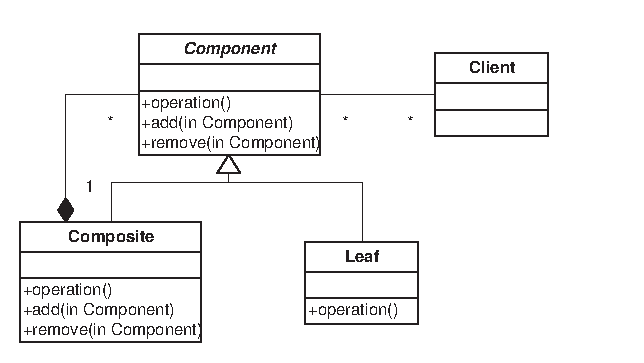
\includegraphics[scale=0.7]{eps/compositum.eps}
       \caption{Composite Pattern}
       \label{composite_figure}
    \end{center}
\end{figure}

\subsubsection{Layers}
\label{layers_heading}

With the help of this pattern, software can be organized in horizontal layers
(figure \ref{layer_figure}). Modules and applications can be separated into logical
levels, whereby these levels should be as independent from each other as possible,
to ensure a high substitutability.

\begin{figure}[ht]
    \begin{center}
       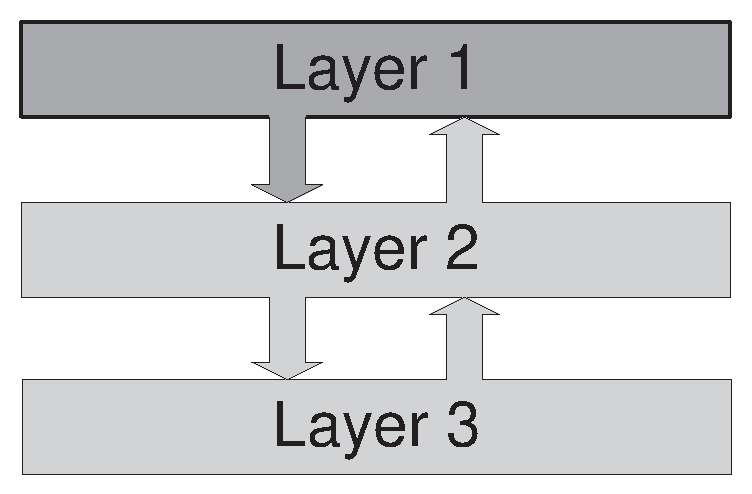
\includegraphics[scale=0.5]{eps/3-Tier-1.eps}
       \caption{Layer Pattern}
       \label{layer_figure}
    \end{center}
\end{figure}

\subsubsection{Chain Of Responsibility}
\label{chain_of_responsibility_heading}

Messages initiated by a particular object can be sent over a chain of instances
to the receiving object (figure \ref{chain_of_responsibility_figure}). So, either
the message will be transmitted over a bunch of objects or evaluated immediately
by the target object.

\begin{figure}[ht]
    \begin{center}
       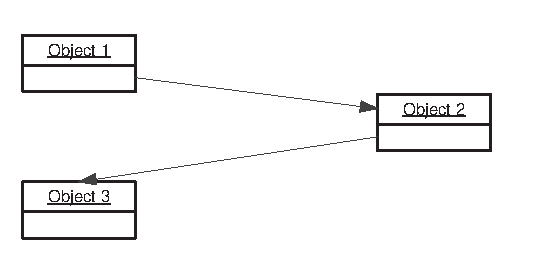
\includegraphics[scale=0.8]{eps/chain.eps}
       \caption{Chain Of Responsibility Pattern}
       \label{chain_of_responsibility_figure}
    \end{center}
\end{figure}

\subsubsection{Model-View-Controller}
\label{model_view_controller_heading}

Dividing the presentation layers into the logical components \emph{Model},
\emph{View} and \emph{Controller}, is a very approved way for designing software
for user interfaces. The model encapsulates the data presented by the view and
manipulated by the controller (figure \ref{model_view_controller_figure}).

\begin{figure}[ht]
    \begin{center}
       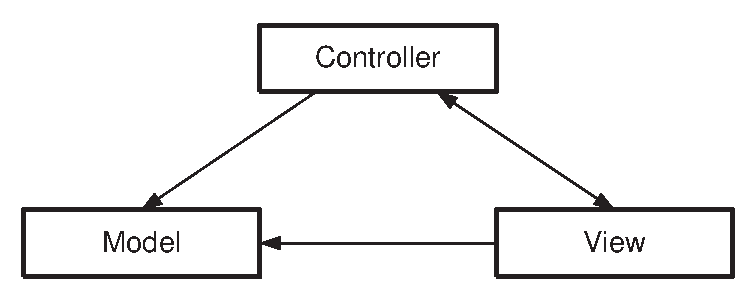
\includegraphics[scale=0.6]{eps/mvc-1.eps}
       \caption{Model-View-Controller Pattern}
       \label{model_view_controller_figure}
    \end{center}
\end{figure}

\subsubsection{Hierarchical Model-View-Controller}
\label{hierarchical_model_view_controller_heading}

The Hierarchical Model-View-Controller \cite{cai} combines the essential design
patterns \emph{Composite}, \emph{Layers} and \emph{Chain of Responsibility}
into one conceptual architecture (figure \ref{hierarchical_model_view_controller_figure}).
This architecture divides the presentation layer into hierarchical sections
containing \emph{MVC-Triads}. The triads conventionally consist of model, view
and controller parts. Triads communicate with each other by relating over their
controller object.\\
Here is a short explanation of this concept, using a practical example:
The upper-most triad could represent a dialog and the middle one a container
such as a panel. In this container, a third triad -- for example a button --
could be held.

\begin{figure}[ht]
    \begin{center}
       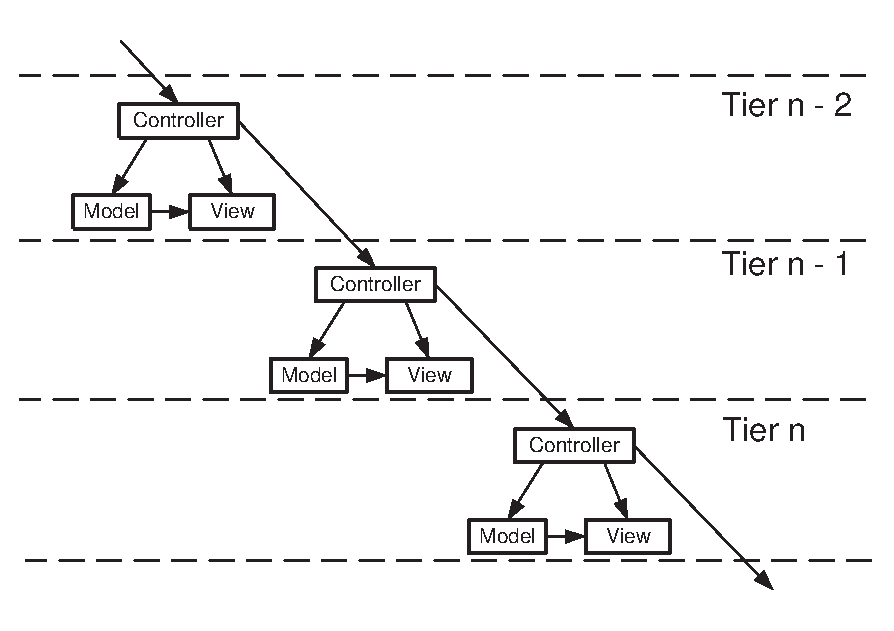
\includegraphics[scale=0.5]{eps/hmvc.eps}
       \caption{Hierarchical Model-View-Controller Pattern}
       \label{hierarchical_model_view_controller_figure}
    \end{center}
\end{figure}

\subsection{Component Lifecycle}
\label{component_lifecycle_heading}

Each \emph{Component} lives in a system that is responsible for the component's
creation, destruction etc. When talking about components, this article sticks
to the definition of Apache-Jakarta-Avalon \cite{jakarta}, which considers
components to be \emph{a passive entity that performs a specific role}.\\
A component has a number of methods which need to be called in a certain order.
The order of method calls is what is known as \emph{Component Lifecycle}.
An outside, active entity is responsible for calling the lifecycle methods
in the right order. In other words, such an entity or \emph{Component Container}
can control and use the component. The Avalon documentation \cite{jakarta} says:

\begin{quotation}
    \textit{
        It is up to each container to indicate which lifecycle methods it will honor.
        This should be clearly documented together with the description of the container.
    }
\end{quotation}

